\section{Mini-MAC}
%The best solution, in that it is implementable and does not change the network infrastructure, to preventing replay and masquerade attacks on the CAN bus to this point is the work presented in Lin-MAC. The underlying MAC protocol was not described, however, and as the ECUs on this node are time-, memory-, and processing power-constrained, some testing must be done to determine which construction is the most suitable for the environment. HMAC is by far the most famous and most popular MAC construction, so three variants of HMAC (that is, HMAC with three underlying keyed-hash functions) were selected for consideration for this project. HMAC is widely used for two key reasons. 1) The security of HMAC is mathematically related to the security of the underlying hash function, which makes it relatively easy to trust and 2) it is extremely easy to plug in various hash functions, making it easy to update to a new implementation if issues are found in the currently used hash\cite{HMAC}\cite{FIPS-198-1}. They are implemented in C on the MSP430.

%The equation for calculating the HMAC is as follows: 

$$ \text{HMAC} = H((K_0\oplus \text{opad})\vee H((K_0\oplus \text{ipad})\vee \text{message}) $$

%Where $K_0$ represents the key, which is sized depending on the underlying hash, and opad and ipad are the outer and inner hash padding strings respectively. These strings are constant strings represented by 0x5C and 0x36 repeated until the hash input string is of the appropriate size. The term $H$ represents the hash function used to generate the HMAC. \cite{FIPS-198-1}

%Figure 1 depicts the key group key distribution model used for Mini-MAC. Note that as multiple ECUs share the same key, messages may be sent to multiple nodes without re-calculating a new MAC for each recipient. This is a key bus overhead reduction compared to Lin-MAC.
	
%	\begin{figure}
%		\centering
%		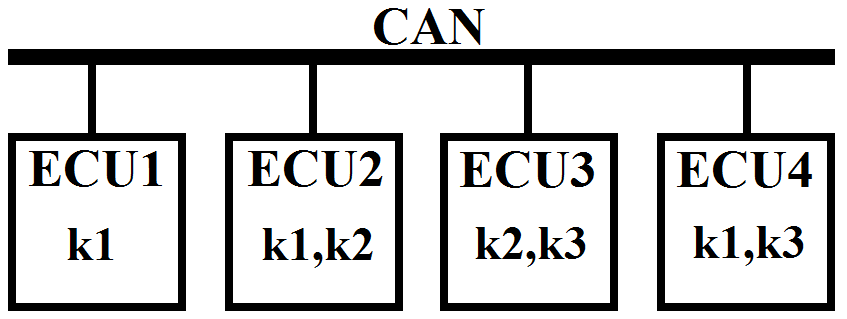
\includegraphics[width=\columnwidth]{figures/key_distribution.png}
%		\caption{Mini-MAC Key Distribution}
%	\end{figure}



A MAC such as the HMAC will defeat the masquerade attack. Legitimate nodes will share some secret key that is used to seed the HMAC and any node without such a key will not be able to create a valid MAC for a given message. However, a standard HMAC will not be able to defeat a replay attack, as the previously recorded message will have a valid MAC. To address this, some time-based token, frequently a counter, can be added to the seeding of the HMAC. The resulting MAC is unique to the message and the time it is sent, which prevents an illegitimate node from simply replaying a message seen in the past.

For the automotive environment, the time-based HMAC has one significant downside - the size of packets on the CAN bus is very small (64B) and the size of the HMAC bit string is, depending on the hash function used, at least twice that size. In order to use normal HMAC, bus traffic would go up some large factor determined by the size of the hash used. 

Mini-MAC is a variable-length Message Authentication Code protocol based on HMAC. It selects an output size to match the available space in a given CAN message. It uses secret keys as well as variable-length counters to seed and condition the HMAC in order to guarantee against repeated MACs.

The core principal of Mini-MAC is that in the automotive environment attackers have a small window of time to break the network. With that in mind, it is possible to design a security mechanism that is capable of defending the network on that very short scale of time without breaking real-time or processing capability constraints.

\subsection{Architecture}

\textcolor{red}{Note: I don't think I have a good understanding of what you mean by architecture vs design. I thought that the third draft had a good balance of high level description vs how the mini-mac is actually constructed. what's left in this draft is a cut-down version of draft 3 as you noted it was not concise}
%Mini-MAC uses group-shared keys (Figure 2) instead of pairwise keys. The use of group keys means that a message need be sent only once and the entire group which needs the message can verify the sender rather than having a separate MAC sent for each recipient. This means Mini-MAC does not need to send any additional  messages in order to provide authentication, which meets the design requirement for bus traffic overhead. Group key distribution is possible because at the time of system design the engineers know exactly which ECUs will need to communicate with which others. There does not need to be a dynamic group update function as there are no circumstances in which a group should change.

Mini-MAC uses group-shared keys (Figure 2) instead of pairwise keys. The use of group keys means that a message need be sent only once and the entire group which needs the message can verify the sender rather than having a separate MAC sent for each recipient. This means Mini-MAC does not need to send any additional message in order to provide authentication, which meets the design requirements for bus traffic overhead. Group key distribution is possible because at the time of system design the engineers know exactly which ECUs will need to communicate with which others. There does not need to be a dynamic group update function as there are no circumstances in which a group should change.

Two counters are used to alter and select the final MAC from the HMAC. The message counter is used to seed the HMAC, while the rollover counter is used to select the starting bit in the HMAC from which the Mini-MAC is drawn.

Message traffic history is used as a post-HMAC confusion step -- the previous messages sent on the sender's ID are used to change the resulting HMAC. This prevents the same MAC being used after the counters roll over. Unless the same message (or message pattern) is repeated exactly, the same MAC will not be issued, even on identical counter values.

Figure 2 depicts the key group key distribution model used for Mini-MAC. Note that as multiple ECUs share the same key, messages may be sent to multiple nodes without re-calculating a new MAC for each recipient. This is a key bus overhead reduction compared to Lin-MAC.
	
	\begin{figure}
		\centering
		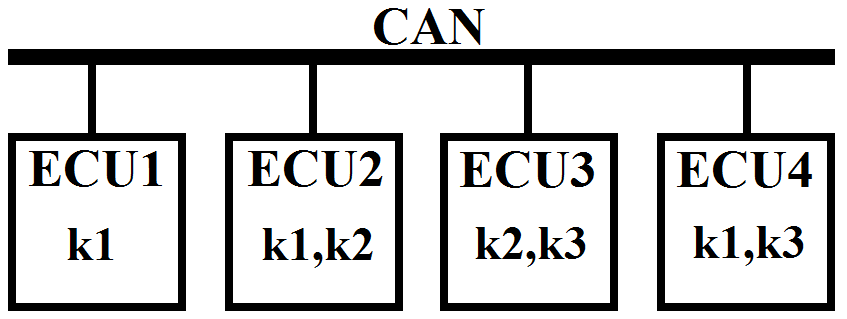
\includegraphics[width=\columnwidth]{figures/key_distribution.png}
		\caption{Mini-MAC Key Distribution}
	\end{figure}
	
	
\subsection{Design}
\textcolor{red}{Note: I don't have a solution to dealing with faults at this time. I believe there are some good ideas in previous work that I will take another look at}

The calculation of Mini-MAC is only slightly more involved than in the HMAC construction. It is shown below:

$$ \text{Input} = \text{Message}_n\oplus\text{Counter}_{\text{msg}} $$
$$ \text{MAC}_{\text{full}} = \text{HMAC}(\text{Input}) $$
$$ \text{For }i=1:h \text{, MAC}_{\text{full}}\oplus\text{Message}_{n-i} $$
$$ \text{MAC}_{\text{mini}} = \text{MAC}_{\text{full}}[l:l+s] $$

\textcolor{red}{Note: One comment was that this section needs to be more precise, but I am unsure how to be more precise than the preceeding formulae -- are they poorly formed? To me, it is quite clear but I understand if they don't appear that way from a different perspective.}

\textcolor{red}{You note that h, l and s are undefined, but they are defined below:}

Where $n$ is the number of the message in a sequence of messages, $n=0$ being the most recent message, $h$ is the number of messages from history to be used for MAC confusion, $l$ the starting bit to pull the Mini-MAC from, and $s$ being the size of the Mini-MAC in bits. The value of $l$ is determined by a second counter designated the rollover counter, which ticks when the message counter rolls over. The result of this two-counter system is that a new MAC is generated for each value of the message counter, and from that MAC, the bits starting with the bit addressed by the rollover counter are taken as the Mini-MAC. This way, when the message counter rolls over, the bit start location shifts so the same Mini-MAC is not re-used until the rollover counter rolls over.

\subsection{Implementation}
One of the most important aspects of HMAC is that it allows the use of a wide range of iterative hash functions as its base. Mini-MAC, being based on HMAC itself, similarly allows various hash functions as a base. HMAC with three common hash functions were used to compute the Mini-MAC for this work. Their varying performance and security characteristics provide end users with a spectrum of solutions to choose from without needing to vary the Mini-MAC computation.

\textcolor{red}{Note: Adapting the original code for the MSP430 is mostly a matter of type conversion- the MSP430 is a 16 bit device, but most of the code is written for 32 bit systems. I don't want to spend more time discussing the hash implementations than necessary as they aren't really important to the end system -- what we do with the HMAC after it's computed is the important part. I added the paragraph above to explain why I used various hashes}

\textbf{HMAC-MD5}
The MD5 implementation tested for this project was originally written by Alexander Peslyak \cite{Peslyak} and adapted for the MSP430 platform by the authors. \\-------\\
Alexander Peslyak \cite{Peslyak} wrote the original MD5 implementation used in this project, and it has been adapted for use on the MSP430 platform by the authors. 

MD5 produces a 128-bit output value from a variable length message. Since 2004, the security of MD5 has been severely compromised \cite{Wang-MD5} -- however, tests showed that it was the fastest HMAC construction and for that reason only it was used as a basis for Mini-MAC. It should be noted that any other hash function could be used, but the test was interested in computation speed more than any other metric\cite{MD5}.

\textbf{HMAC-SHA1}
The HMAC-SHA-1 implementation used for this project was originally written by Brad Conte \cite{Conte-SHA1} and adapted for the MSP430 platform by the authors. SHA-1 produces a 160-bit output value from variable length inputs. Similar to MD5, security vulnerabilities have been found in SHA-1 \cite{Wang-SHA1}, but it is still used in many applications and will be for the immediate future\cite{FIPS-180-4}.

\textbf{HMAC-SHA256}
The HMAC-SHA-256 implementation used in this project was originally written by Brad Conte \cite{Conte-SHA256} and was adapted for the MSP430 platform by the authors. SHA-256 is a member of the SHA-2 family of hash functions. This family produces fixed length output values from variable length input sequences. SHA-2 is still in use and is recommended by NIST as a secure hash function, but SHA-3 will soon replace it\cite{FIPS-180-4}.